%===================================== CHAP 5 =================================
\section{Laser Annealing of Fibers}
\section{Fabrication of Electrical Contacts on Fibers}

In this work we wish to perform electrical characterization of fiber cores. Due to the small dimensions of the fiber core, this requires the patterning of metal contacts with micrometer scale resolution and similar alignment accuracy with the fiber core. This is achieved through the use of maskless lithography and a liftoff procedure using physical vapor deposition.% Fibers are patterned by maskless lithography, followed by deposition of thin films using physical vapor deposition (PVD). The resist is then removed by liftoff leaving the desired metal contacts. 
 

\subsection{Overview of Maskless Lithography}
%possible diamgram of liftoff process.
Maskless Lithography, or direct laser writing (DLW) is an emerging form of lithography that allows for patterns to be directly written from a digital image to the resist layer without the use of a conventional photomask. Patterns are exposed using a UV laser and a digital micromirror device (DMD), achieving a minimum feature size under $1 \si{\micro\meter}$. Compared to Electron Beam Lithography (EBL), a staple of nanofabrication, maskless lithography greatly decreases the writing times and is compatible with conventional resists used for UV lithography. 

Direct laser writing has several major advantages over conventional lithography for patterning on fibers. The use of a digital pattern allows for customization of the contact pattern for each individual fiber. As the fiber diameter and available lengths of continuous core varied, it was necessary to adjust the pattern to obtain an optimal contact spacing, and space the contacts in available areas between cracks in the core. The MLA150 and MLA100 allow for the pattern to be alligned with the substrate with $\SI{500}{\nm}$ accuracy. This allows for precise positioning of the pattern with the fiber cores. 

For this study an MLA150 maskless alligner from Heidelberg instruments with $\SI{375}{\nm}$ and $\SI{405}{\nm}$lasers is primarily used. Alternatively a Heidelberg MLA100 with $\SI{10}{\watt}$ $\SI{365}{\nm}$ UV LED. A resolution test, shows the ability to achieve $ 1 \si{\micro \meter}$ features in man-440 resist \ref{fig:resolution_test}. 

\begin{figure}[!htb]
    \centering
    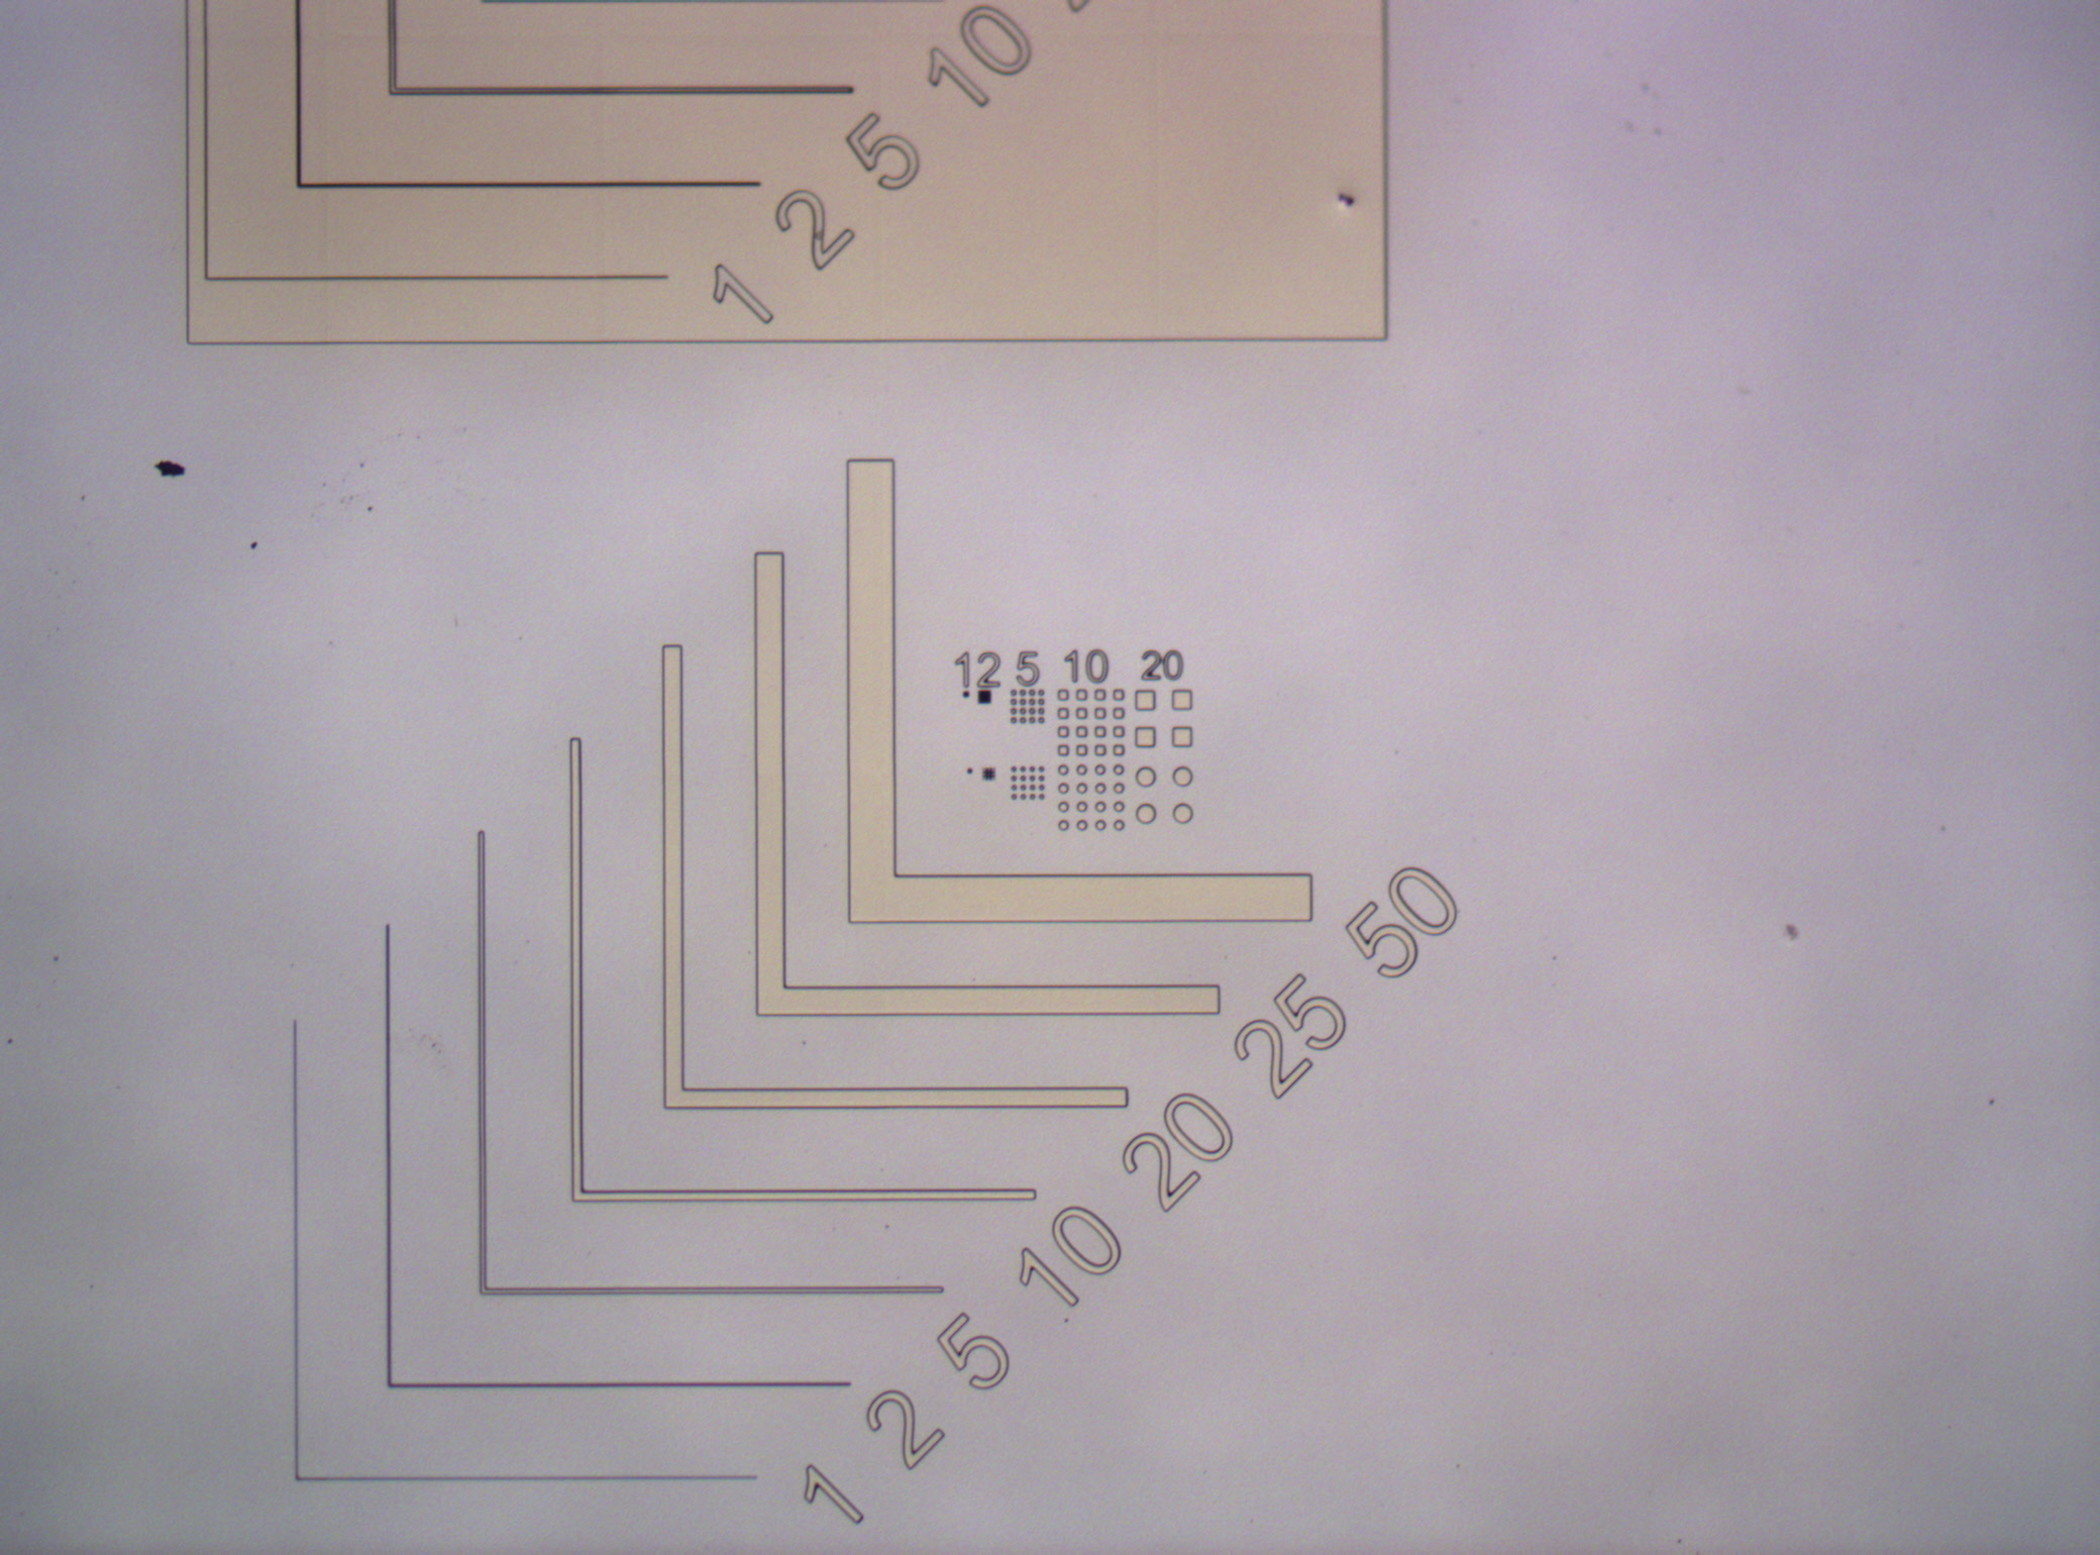
\includegraphics[width=\textwidth]{fig/Results/resolution_test.jpg}
    \caption{Resolution test with Man-440 photo resist on a Si wafer exposed at  $\SI{3200}{\milli \joule \cm^{-2}}$ at $\SI{365}{\nm}$. The numbers indicate the width of the line in microns, and the top of the image shows negative structures, while the bottom shows positive lines on the grey Si background.}
    \label{fig:resolution_test}
\end{figure}


\subsubsection{Choice of Photoresists}

 \begin{figure}[!htb]
    \centering
    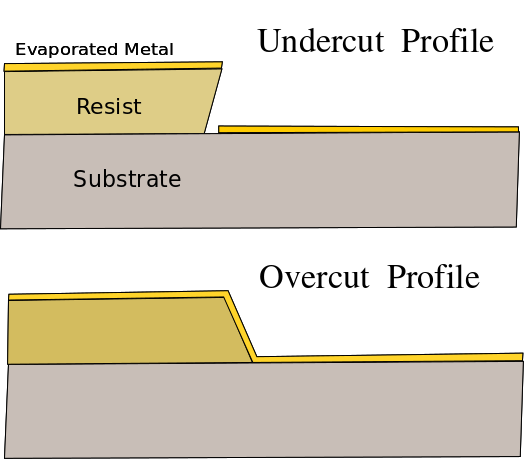
\includegraphics[width=.5\textwidth]{fig/Methods/resist_profile_2.png}
    \caption{}
    \label{fig:resist_profile}
\end{figure}

In lithography, the resist is a photosensitive chemical that changes it's solubility on exposure to UV light. Resists can either be positive or negative which describes whether the exposed resist will become soluble or insoluble respectively. Positive resists form  indene carboxylic acid making them soluble, while negative resists cross-link on exposure making them insoluble and thermally stable. Higher temperatures increase the degree of cross-linking making the resist more difficult to remove from the substrate. A significant difference between positive and negative resists is the sidewall profile . During exposure the top layer of resist becomes more highly irradiated thus creating a gradient in the solubility across the resist thickness, this tends to create overcut profiles in positive resists and undercut profiles in negative resists (see figure \ref{}). For a liftoff procedure using PVD this undercut profile prevents the resist sidewalls from becoming coated in metal which allows for easier removal of the resist in solvent. 

While the thickness of the resist is generally chosen based on the desired thickness of the deposited metals, the samples in this work were not perfectly planar due to relief between the glass cladding and epoxy that arises during polishing due to differences in hardness. As this relief was up to several micrometers in height Man-440 negative resist was chosen for this work. This resist is designed for a thickness of $\SI{4.1}{\micro \meter}$ which can safely accommodate the height variations of the sample surface and provides easy lift-off in organic solvents. The Man-440 resist showed good adhesion to epoxy substrate, while an adhesion promoter such as HDMS was suggested for use on silicon and glass. This proved not to be an issue on fibers due to the large feature size of the contact designs, however, small unsupported features such as thin lines on Si and glass occasionally delaminated from the surface. A test was performed of other available resists in this thickness range but none showed suitable liftoff times. [Table of resists here] 


\subsection{Development of resist Recipe}
The resist was applied by spin-coating at $3000$RPM for $33 \si{\sec}$ with $500$ RPM/s. A prebake is then performed to remove excess solvent from the resist. A prebake time and temperature is suggested of $\SI{95}{\celsius}$ and $\SI{300}{\second}$ for a contact hotplate and $\SI{100}{\celsius}$ for  $\SI{30}{\minute}$ in an oven.  Due to the thickness of the substrate and lower thermal conductivity as compared to a Si wafer an oven bake at the suggested values was used. However these results led to substantially longer development times. It was found that a prebake on a contact hotplate gave good results, indicating that the prebake was not extremely sensitive to the sample thickness and thermal conductivity. 

\subsubsection{Exposure}
The resist is activated by exposure to UV light, and has sensitivity that depends on wavelength. The exposure dose further depends both on the resist thickness and reflectively of the substrate. The optimal dose was determined by exposing a test structure multiple times with varying energy, as seen in figure \ref{fig:resolution_test} and comparing the pattern after development. With this method the optimal dose was found to be $\SI{3200}{\milli \joule \cm^{-2}}$ at $\SI{365}{\nm}$ or $\SI{2400}{\milli \joule \cm^{-2}}$ at $\SI{405}{\nm}$. 

\subsubsection{Development}
 The resist was developed using micro-chemicals ?? developer. It was found that the development time varied greatly depending on the time the bottle was first opened and ranged from $160-210 \si{\second}$, which is described further in the results section {}. After development the sample was rinsed with deionized water for $30 \si{seconds}$ to remove any remaining solvent and dissolved resist and dried with nitrogen. 
 

 To ensure a clean surface and promote proper adhesion of the deposited contacts, a plasma clean was used after development using a Diener Electronics Femto plasma cleaner. A plasma clean of $1 \si{\minute}$ at $50\si{\watt}$ power using $50\%$ oxygen flow.   Plasma cleaning can also remove the cross linked resist thus the resist height was checked with a stylus profilometer before and after cleaning. No noticable removal was found for the cleaning times used. 
 
 \subsection{Physical Vapor Deposition and Liftoff}
 


Contact Deposition was performed using an AJA International Inc. Custom ATC-2200V sputter coater and evaporator. During E-beam evaporation a electron beam is used to evaporate material from a source target, which is then deposited onto the sample surface. Multiple targets can be used sequentially deposit layers of different materials. With sputtering, a plasma is created and ions are accelerated into the target to eject material. Sputtering produces atoms with higher kinetic energy and due to scattering of the sputtered atoms off of gas molecules, there is better step coverage on the sample.

To promote easy lift-off contacts of were deposited using E-beam evaporation due to its lower step coverage. $5 \si{\nano\meter}$ of Ti was first deposited to promote adhesion to the substrate followed by  $100 - 200\si{\nano\meter}$ Au. The sample was rotated to promote uniform coverage. Liftoff of the resist was performed by submersion in an acetone bath for several minutes followed by sonication if necessary. Liftoff times varied likely as a result of variation in the undercut of the resist. Development time was therefore an important parameter to optimize to avoid excessive time in acetone or long sonication times which could lead to delamination of the contacts. 

A summary of all the steps in the complete process for contact deposition is given in table \ref{Tab:recipe}.

\begin{table}[h]
\begin{center}
    \begin{tabular}{|l|l|  }
    \hline
    \textbf{Process Step} & \textbf{Parameters} \\ \hline
    Sample Cleaning & Sonication in Acetone followed by rinse in ethanol and IPA. \\ 
    &Plasma cleaning $100 \si{\watt}$  $100\%$ $\mathrm{O_2}$ for $ \SI{2}{\minute}$\\ \hline
    Spin Coating & $300$ RPM for $\SI{33}{\second}$ with $500$ RPM/s acceleration. \\ \hline 
   Prebake & $\SI{95}{\celsius}$ for $\SI{300}{\second}$ on a contact hoplate. \\ \hline
   Exposure & $\SI{3200}{\milli \joule \cm^{-2}}$ at $\SI{365}{\nm}$ using MLA100 \\
   & $\SI{2400}{\milli \joule \cm^{-2}}$ at $\SI{405}{\nm}$ using MLA150 \\\hline
   Development & $160-210 \si{\second}$ using ?? \\ \hline
   Plasma Ashing & $1 \si{\minute}$ at $50\si{\watt}$ power using $50\%$ $\mathrm{O_2}$ flow\\ \hline
   Deposition &  E-beam evaporation of $\si{\nano\meter}$  Ti /  $100 - 200\si{\nano\meter}$    \\\hline
   Liftoff & Several minutes in an Acetone bath. Sonication if necessary. \\ \hline
    \end{tabular}
\end{center}
\caption{A full process recipe for the deposition of Ti/Au contacts }
\label{Tab:recipe}
\end{table}

 
 

\subsection{Permanent Resist Underlayer}  \label{permanentunderlayer} %should it be its own section?
\begin{figure}[!htb]
    \centering
    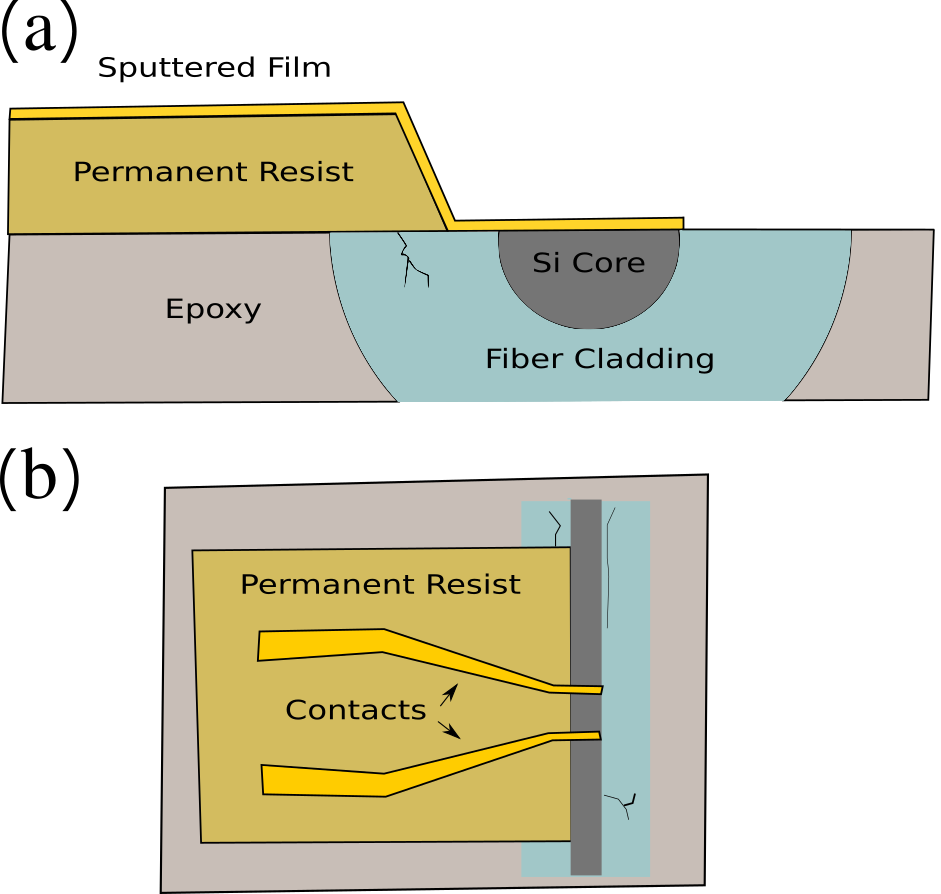
\includegraphics[width=.7\textwidth]{fig/Methods/permanentresist_test.png}
    \caption{(a) Profile view of a permanent resist layer used to cover cracks in the fiber cladding to allow for continuous contact to be made to the fiber core. (b) Top view of the same illustration showing two contacts. On a realistic sample, multiple contacts will be made to the core for four terminal and hall measurements. Note images not to scale. }
    \label{fig:permanentresist}
\end{figure}
In order to measure the fiber core it was necessary to deposit a continuous conductive film with a thickness of only $100-200 \si{nm}$. As mentioned in section \ref{ovenanneal} cracking of the fiber cladding during polishing, was a common occurrence and would therefore break the continuity of a deposited contact. It was common to see a parallel crack propagating on at least one side of the core, with cracking becoming more severe in samples with a larger core to cladding ratio, and in hand drawn samples. Not only does this limit the contact spacing and the number of measurements that can be made on one sample, it also affects the ability to make hall measurements, as the hall pattern requires contacts on either side of the fiber. If we desire to create structures or junctions within the fiber and characterize the core at the exact point the chances of cracking preventing measurement of the fiber are substantially higher. Due to the small size of the cracks, it is unlikely that filling them with a method such as vacuum impregnation with epoxy would be successful. Further this would require a second polishing step to remove this new layer from the core for electrical measurements.

While photoresist is mainly used for masking purposes, adding a permanent layer of resist would create a smooth surface for the deposition of contacts. The resist can be patterned to leave only the fiber core exposed, and integrates easily with the current process  as a second lithography step would add little to the preparation time. The challenges are that the resist layer must be stable in solvent during a second liftoff process and that the contacts deposited over the resist, adhere well and can create continuous coverage of the resist step edge. For the latter a positive resist would be the ideal choice due to the positive sidewall profile. Further a greyscale resist such ma-p1275g  would allow thick films (~100 um) and a controllable positive sidewall profile. While ma-p1275G would be an ideal choice, tests showed that it was stable enough after hard baking to withstand an acetone bath. 

The negative photo resists $SU-8$ and $mr_DWL$ are epoxy based and designed for creating high aspect ratio structures with nearly vertical sidewalls. Further a hardbake step up to 140C creates a very stable resist. While the sidewall profile is still negative, tilting the sample during depostion, or using sputtering may allow sufficient step coverage to create a continuous contact. 

\subsubsection{Experimental Procedures}
A test sample using mr-DWL 5 was patterned on a Si wafer using the following parameters: spin 3000 rpm patterning $\SI{500}{\milli \joule \cm^{-2}}$ at $405 \si{\micro\meter}$ in the MLA, followed by a hard bake of 30 min $140 \si{\celsius}$. This structure was then coated with $\SI{4}{\micro \meter \cm^{-2}}$ man-440 using the standard recipe described above. 

The procedure was tested on a fiber to examine how the process would work under practical conditions, as the resist thickness, bake temperature and reflections during exposure would all be slightly effected. Electrical contacts were deposited using the standard recipe followed by a sputtered layer of $100 \si{\nano \meter}$. After electrical testing, a further layer of Au was deposited by sputter coating in a small cressington 208 HR B sputter coater, as this was the only method of deposition that allowed for tilting of the sample. Both test samples were analysed by 3d-optical profilometry and SEM. 

\section{Characterization techniques}
\subsection{Four point probe }
Four point probe measurements were performed with a Dectak ... with a Signatone SP4 head with 1 millimeter probe spacing and ?? radius tips.

\subsection{Electrical Measurements with MiBots}
An alternative to the Lithographic techniques described, is direct probing of the sample using micro manipulators. In this work Imina Techinology Mibots are used to perform four point measurements of fiber cores. MiBots are vacuum compatible micro manipulators with interchangeable tungsten probes capable of electrical probing. The probe positioning precision is in the $\si{nm}$ range and is more than sufficient for fiber measurements. The MiBots have a stage that can be used with an optical or electron microscope. 

Direct probing has the advantage of eliminating the challenges associated with lithography, including the need to bridge an cracking in the glass fiber and any relief profile and possible chipping at the glass epoxy interface. Problems with metal adhesion to the three different materials (glass,epoxy,core) are substrate is also eliminated. While work has been done to use micro manipulators to characterize semiconductor fibers \cite{Engel2016DirectPhotosynthesis} past experience in our group has found that reliable electrical contact is difficult to achieve. %Ohmic contacts of the manipulators requires sufficient force (look up here). 

In this work micro contacts along the core providing a reliable method of contacting the sample. Measurements are performed under an optical microscope with $20\times$ magnification. A ?? source meter is used to perform current sweep measurements of $-1 \si{\milli\ampere}$ to $1 \si{\milli\ampere}$ with the current sweeping up from lowest to highest values, and back down to the starting value to reveal any hysterisis in the measurement. Two point measurements are performed between the individual probes to check whether the contacts are ohmic. 



\begin{figure}[t]
  \centering
    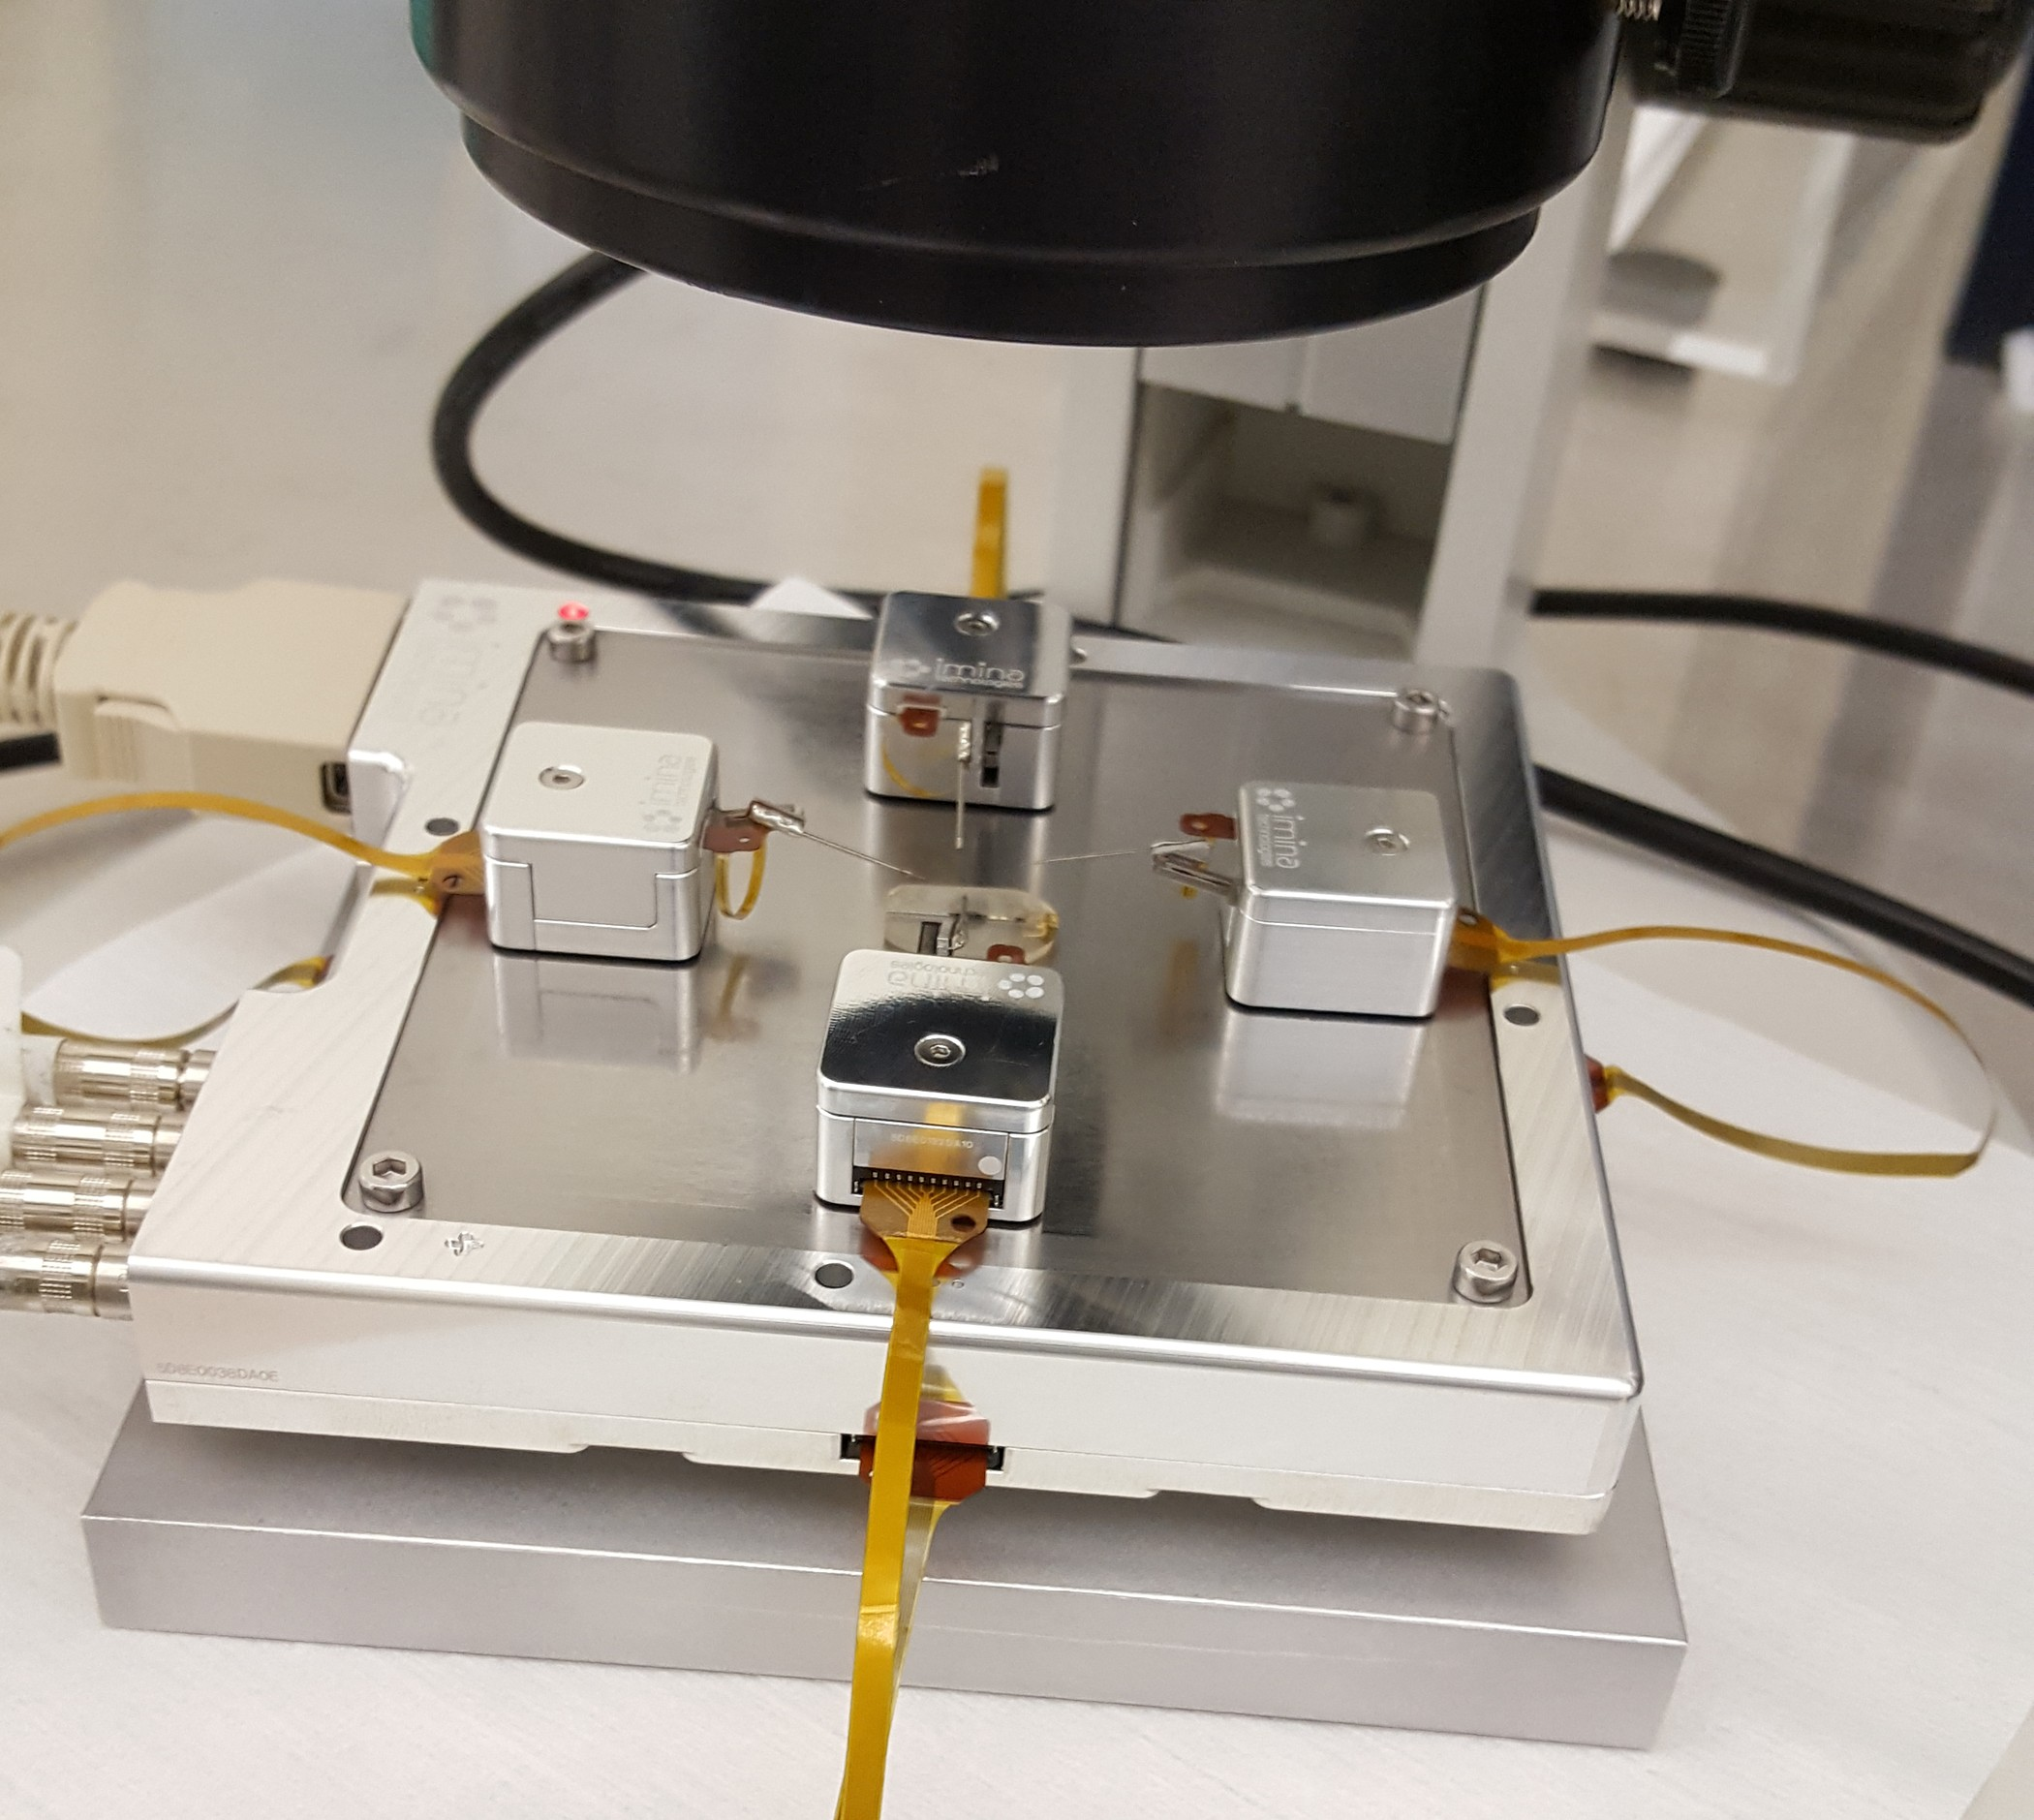
\includegraphics[width=0.7\textwidth]{fig/MiBots/setup.jpg}
 \caption{}
\label{mibot}
\end{figure}

\begin{figure}[t]
  \centering
    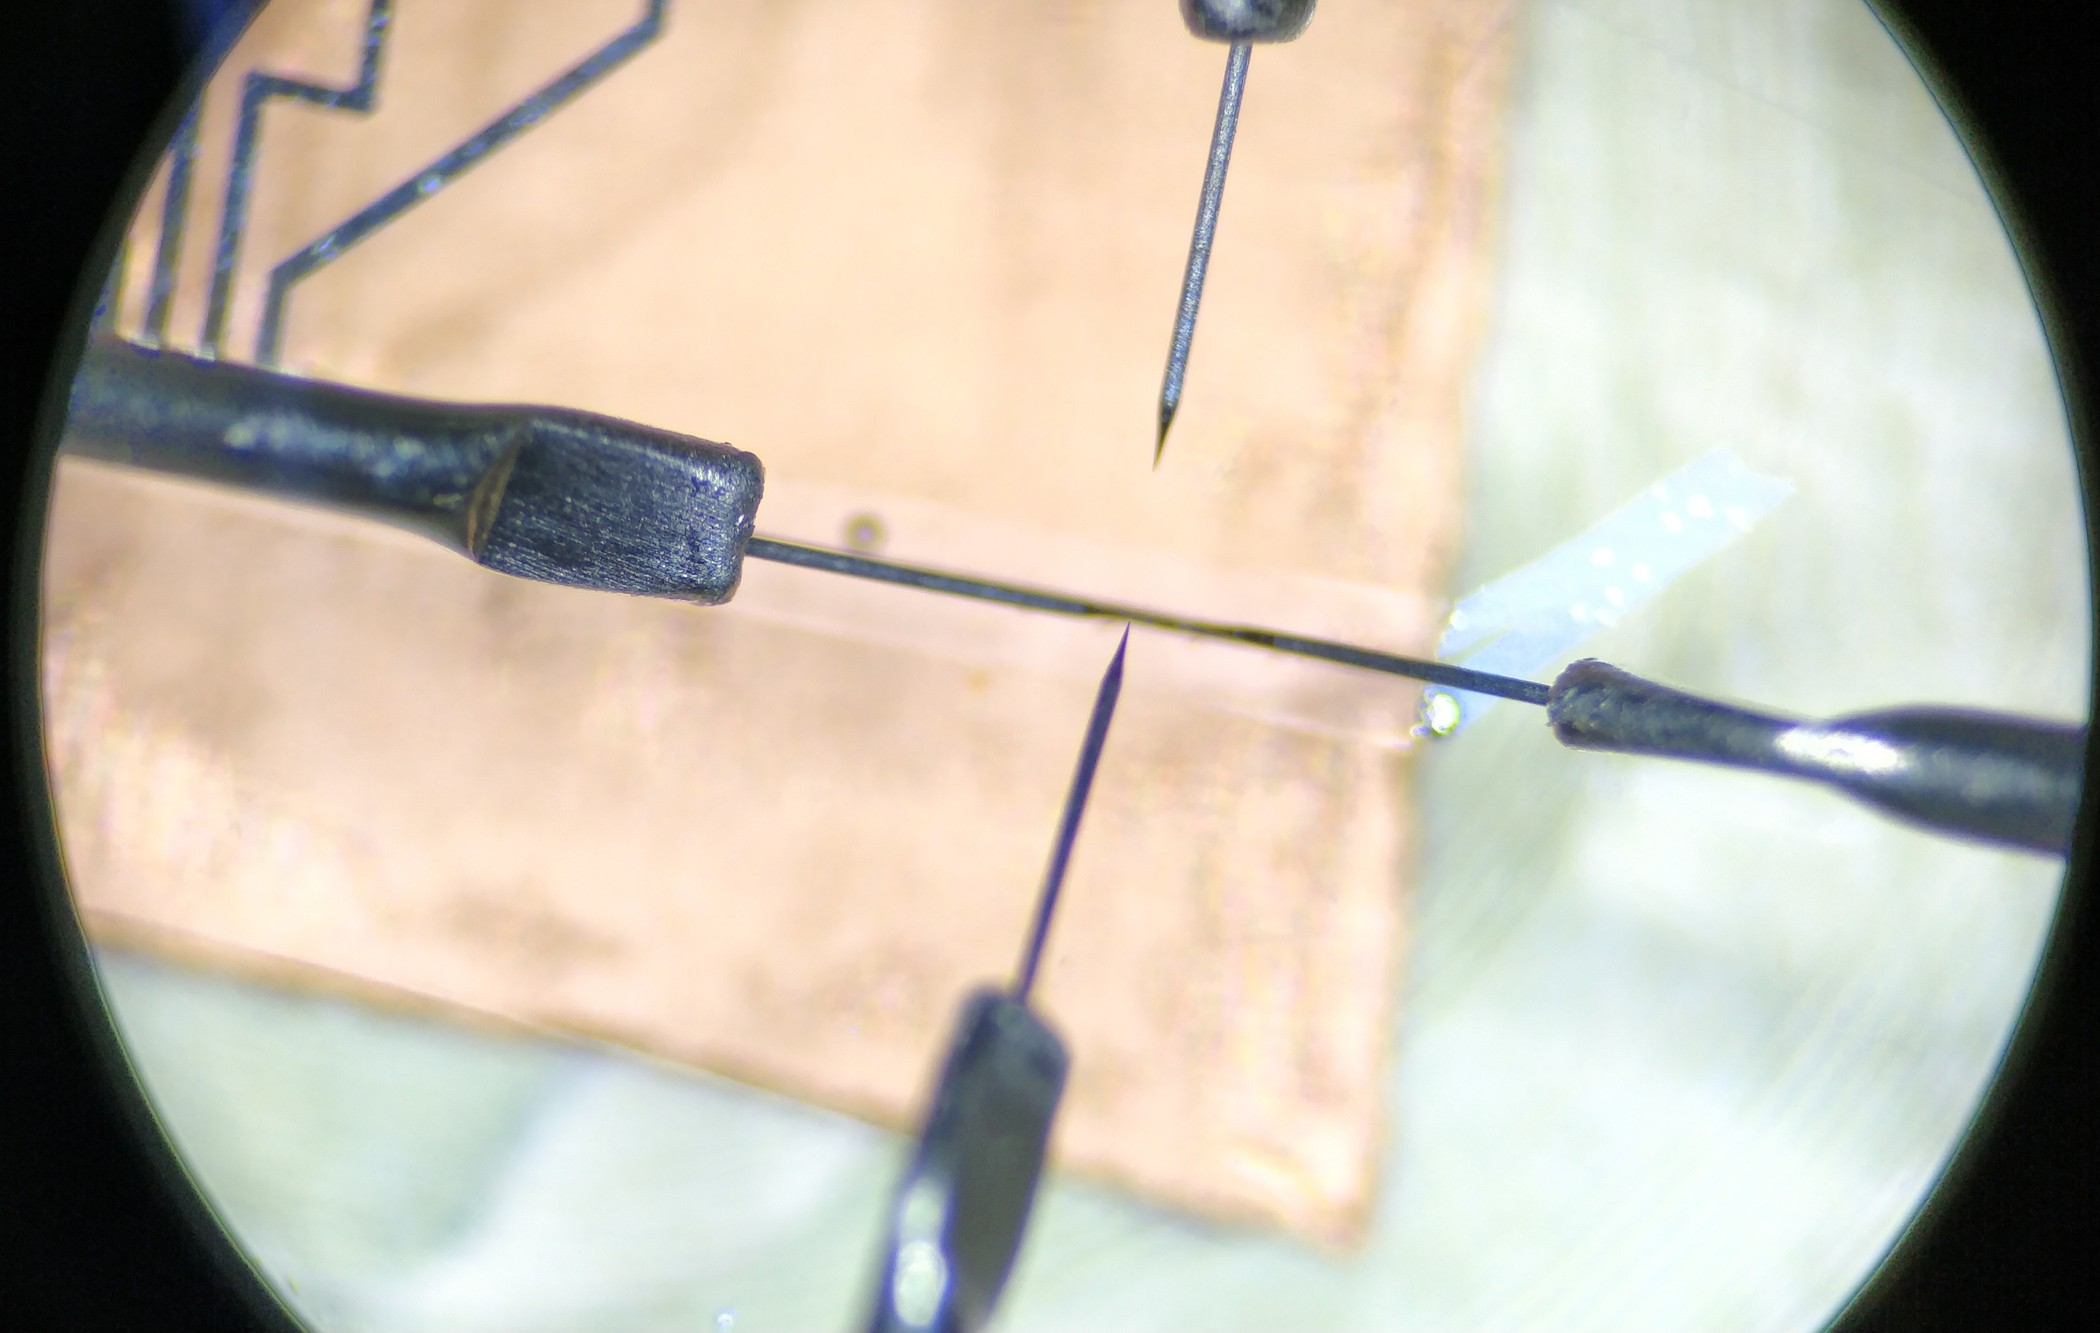
\includegraphics[width=0.7\textwidth]{fig/MiBots/IMG_20190409_143016.jpg}
 \caption{ Mibot with 1 um Probe tips directly contacting the exposed sample core. The two outer current carrying probes are in contact while the voltage probes are raised above the sample.}
\label{mibot1}
\end{figure}


%\begin{fgure}[h]
%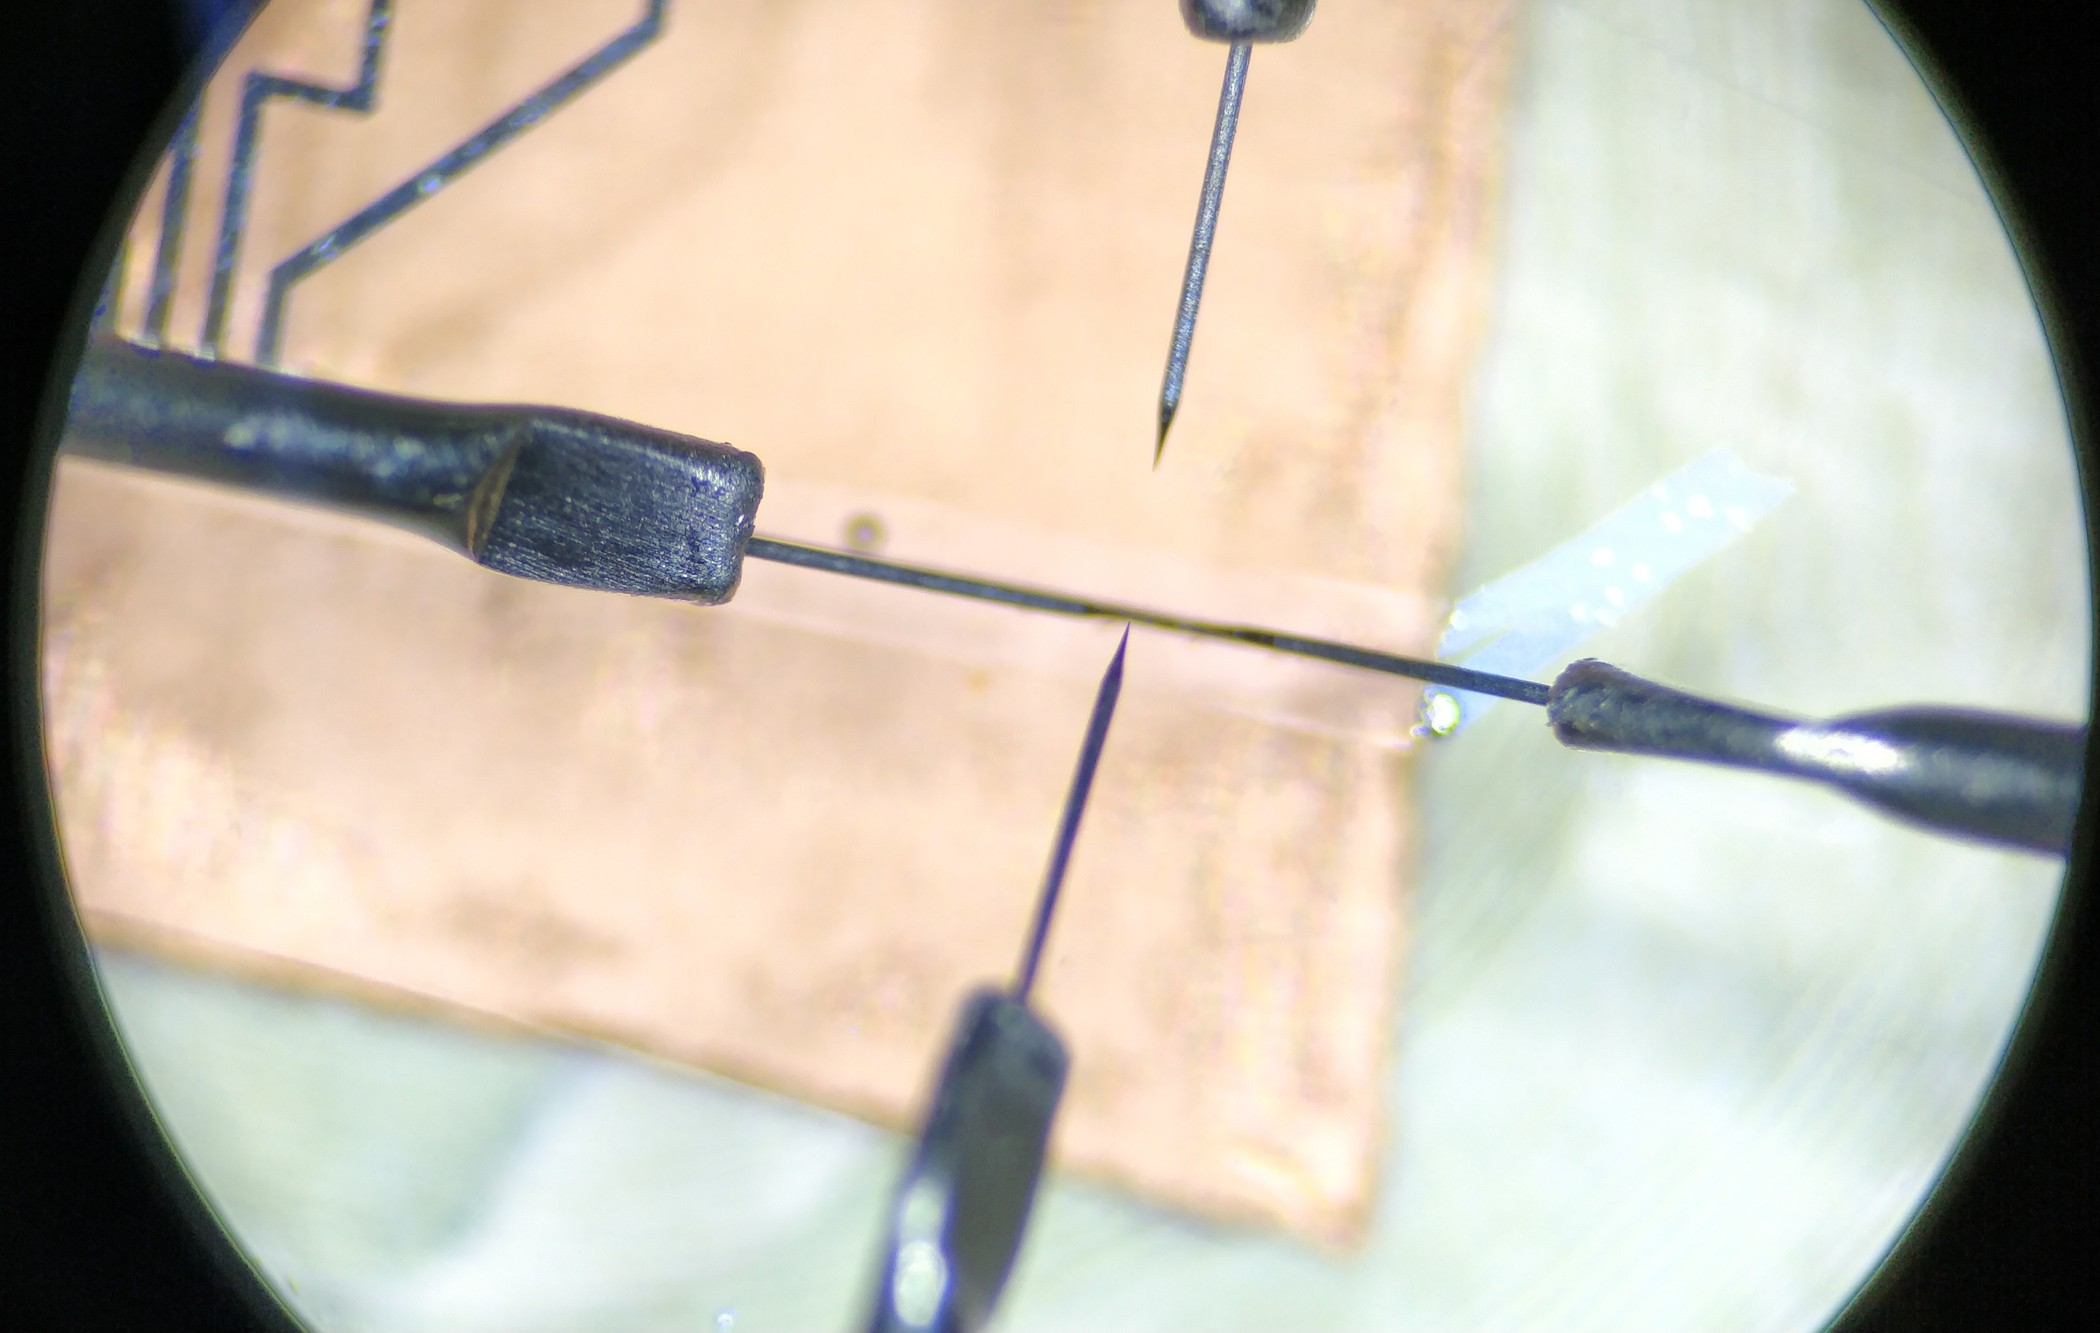
\includegraphics[width=.7\textwidth]{fig/MiBots/IMG_20190409_143016.jpg}
%\caption{Mibot with 1 um Probe tips directly contacting the exposed sample core. The two outer current carrying probes are in contact while the voltage probes are raised above the sample.}
%\end{figure}

\subsection{Profilometry}
\subsection{Scanning Electron Microscopy}
\cleardoublepage